% Template for a Computer Science Tripos Part II project dissertation
\documentclass[12pt,a4paper,twoside,openright]{report}
\usepackage[pdfborder={0 0 0}]{hyperref}    % turns references into hyperlinks
\usepackage[margin=25mm]{geometry}  % adjusts page layout
\usepackage{graphicx}  % allows inclusion of PDF, PNG and JPG images
\usepackage{verbatim}
\usepackage{pdfpages} % allows inclusion of non tex project proposal
\usepackage{docmute}   % only needed to allow inclusion of proposal.tex

\raggedbottom                           % try to avoid widows and orphans
\sloppy
\clubpenalty1000%
\widowpenalty1000%

\renewcommand{\baselinestretch}{1.1}    % adjust line spacing to make
                                        % more readable
\begin{document}

\bibliographystyle{plain}


%%%%%%%%%%%%%%%%%%%%%%%%%%%%%%%%%%%%%%%%%%%%%%%%%%%%%%%%%%%%%%%%%%%%%%%%
% Title


\pagestyle{empty}

\rightline{\LARGE \textbf{Oliver Black}}

\vspace*{60mm}
\begin{center}
\Huge
\textbf{Software IPv6 Router in Rust} \\[5mm]
Computer Science Tripos -- Part II \\[5mm]
Selwyn College \\[5mm]
\today  % today's date
\end{center}

\newpage
\section*{Declaration of Originality}

I, Oliver Black of Selwyn College, being a candidate for Part II of 
the Computer Science Tripos, hereby declare
that this dissertation and the work described in it are my own work,
unaided except as may be specified below, and that the dissertation
does not contain material that has already been used to any substantial
extent for a comparable purpose.

\bigskip
\leftline{Signed Oliver Black}

\medskip
\leftline{Date \today}

%%%%%%%%%%%%%%%%%%%%%%%%%%%%%%%%%%%%%%%%%%%%%%%%%%%%%%%%%%%%%%%%%%%%%%%%%%%%%%
% Proforma, table of contents and list of figures

\pagestyle{plain}

\chapter*{Proforma}

{\large
\begin{tabular}{ll}
Name:               & \bf Oliver Black                      \\
College:            & \bf Selwyn College                     \\
Project Title:      & \bf Software IPv6 Router in Rust \\
Examination:        & \bf Computer Science Tripos -- Part II, July 2001  \\
Word Count:         & \bf "FIX ME\& footnote" \footnotemark[1]
                       \\
Project Originator: & Oliver Black \& Dr Richard Watts      \\
Supervisor:         & Andrew Moore                   \\ 
\end{tabular}
}
\footnotetext[1]{This word count was computed
by \texttt{detex diss.tex | tr -cd '0-9A-Za-z $\tt\backslash$n' | wc -w}
}
\stepcounter{footnote}


\section*{Original Aims of the Project}

The IPv6 standard contains a large number of complex requirements, complicating understanding. I aim to design and implement a simple IPv6 router using Rust\cite{rust} that behaves as specified in the IPv6 RFCs\cite{ipv6_rfc}. This router should implement the minimum functionality required by the relevant standards, yet still be functional, minimal, \& stable.  Rust is a new programming language that aims to be as fast as C while maintaining memory safety, I wanted to understand how practical it was to develop in.

\section*{Work Completed}

Despite having initial difficulties setting up my test environment using Mininet\cite{mininet}, due to its lack of support for IPv6, I successfully implemented a functioning IPv6 router in rust that met almost all of my core requirements. Both the router itself, and the test bench, are available for public use.  TODO mention speedup/code coverage/size/RFC coverage/throughput AND fill rest in when main body done. mention how ambitious original claims were

\section*{Special Difficulties}

None. TODO fill in

\tableofcontents

\listoffigures

\newpage
\section*{Acknowledgements}

Many thanks to:
\begin{itemize}
\item My supervisor Andrew Moore for his helpful advice.
\item My Director of Studies Dr Richard Watts for his guidance.
\item Friends \& family for proofreading.
\end{itemize}

%%%%%%%%%%%%%%%%%%%%%%%%%%%%%%%%%%%%%%%%%%%%%%%%%%%%%%%%%%%%%%%%%%%%%%%
% now for the chapters

\pagestyle{headings}

\chapter{Introduction}
Slowly but surely the internet is making progress towards IPv6, and how do pages of Requests for Comments (RFCs) translate into real world network components. The aim of this project was to develop an IPv6 Router in Rust that explores the functionality of IPv6, and how different parts of the various standards fit together. The project has been a success, I have produced a functioning router and accompanying test suite.

\bigskip

Due to the popularity of the Internet, there are now not enough IPv4 addresses to go around. IPv6 is the incoming internet addressing standard that solves numerous issues with IPv4.  Primarily it increases the number of addresses, however it also fixes many flaws in the IPv4 design, and standardises common non-standard practices. For example, the Time To Live in IPv4 was defined partly in terms of seconds left to live\cite{ipv4_rfc}, but in practice was decremented by 1 every hop between nodes. In IPv6 the field is accurately renamed to Hop Limit, and is now defined in terms of hops between nodes (as opposed to seconds). Many subtle decisions like this have gone into the IPv6 standard, with an aim to making an internet that works well, rather than one that just works.

\bigskip

Rust\cite{rust} is an up and coming modern low level programming language. It aims to match the performance of C++ without sacrificing memory safety, and avoiding garbage collection. It does this through zero-cost high level abstractions such as \textit{ownership} and \textit{lifetimes}. For example, if you pass a struct to a function, that function then owns that struct, with it being inaccessible after the function returns. It is possible for functions to borrow values instead, using "\texttt{\&}", similar to passing by reference.  I chose Rust for my project as it can be easier to debug than C or C++, but mainly because I was interesting in learning Rust.

\bigskip

Mininet\cite{mininet} is an open source virtual network simulator that was developed at Stanford and until 2016 was used in the Part 1B Computer Networking course, it is written in Python.  It creates lightweight virtual networks by making use of Linux's \textit{networked namespaces}, allowing processes to share a kernel, yet be behind different network interfaces. This made it the ideal candidate to build my router and test suite on top of.

\bigskip

Routers are the backbone of the internet, at the most simple level many of them have a \textit{control plane} that deals with addressing, and a \textit{forwarding plane} that deals with sending packets. There are many open source routers out there, but almost all of them have lots of IPv4 code. This makes it difficult to isolate and understand how the IPv6 part actually works.  Starting from scratch allows you to avoid having to deal with IPv4 at all.  Using the IPv6 standard as a framework, combined with some knowledge about the internals of routers, it is possible to develop and IPv6 router that is stable, small, simple, \& fast.

\chapter{Preparation}

Before starting the implementation lots of research and design needed to be done. Lots of research was done into IPv6 RFCs and which aspects were required to be implemented, and which were not. The router software was then designed to provide a framework within which these aspects could be implemented.  Additionally a test plan needed to be made, to enable effective evaluation of the finished product

\section{Research}

\section{Design}

\section{Test Plan}

This chapter is empty!

Examples
Mininet: Ipv4 - see below
Simple Router: https://github.com/mininet/mininet/wiki/Simple-Router

Design
RFCs
Router knowledge - diagram

Test bench
Test criteria (appendix) - spreadsheet
More detail in implementation on mininet


\chapter{Implementation}



\chapter{Evaluation}

\section{Printing and binding}

Use a ``duplex'' laser printer that can print on both sides to print
two copies of your dissertation. Then bind them, for example using the
comb binder in the Computer Laboratory Library.

\section{Further information}

See the Unix Tools notes at

\url{http://www.cl.cam.ac.uk/teaching/current-1/UnixTools/materials.html}


\chapter{Conclusion}

I hope that this rough guide to writing a dissertation is \LaTeX\ has
been helpful and saved you time.


%%%%%%%%%%%%%%%%%%%%%%%%%%%%%%%%%%%%%%%%%%%%%%%%%%%%%%%%%%%%%%%%%%%%%
% the bibliography
\begin{thebibliography}{1}
\addcontentsline{toc}{chapter}{Bibliography}

\bibitem{rust} Rust, a modern low level programming language, https://www.rust-lang.org/
\bibitem{mininet} Mininet, a network virtualisation library in Python, http://mininet.org/
\bibitem{ipv6_rfc} Internet Protocol, Version 6 (IPv6) Specification, RFC 8200, July 2017
\bibitem{ipv6_rfc_adr} IP Version 6 Addressing Architecture, RFC 4291, February 2006
\bibitem{ipv4_rfc} INTERNET PROTOCOL DARPA INTERNET PROGRAM PROTOCOL SPECIFICATION, RFC 791, September 1981
\bibitem{icmpv6_rfc} Internet Control Message Protocol (ICMPv6) for the Internet Protocol Version 6 (IPv6) Specification, RFC 4443, March 2006

\end{thebibliography}

%%%%%%%%%%%%%%%%%%%%%%%%%%%%%%%%%%%%%%%%%%%%%%%%%%%%%%%%%%%%%%%%%%%%%
% the appendices
\appendix

\chapter{Latex source}

\section{diss.tex}
{\scriptsize\verbatiminput{diss.tex}}

\section{proposal.tex}
{\scriptsize\verbatiminput{proposal.tex}}

\chapter{Makefile}

\section{makefile}\label{makefile}
{\scriptsize\verbatiminput{makefile.txt}}

\section{refs.bib}
{\scriptsize\verbatiminput{refs.bib}}


\chapter{Project Proposal}

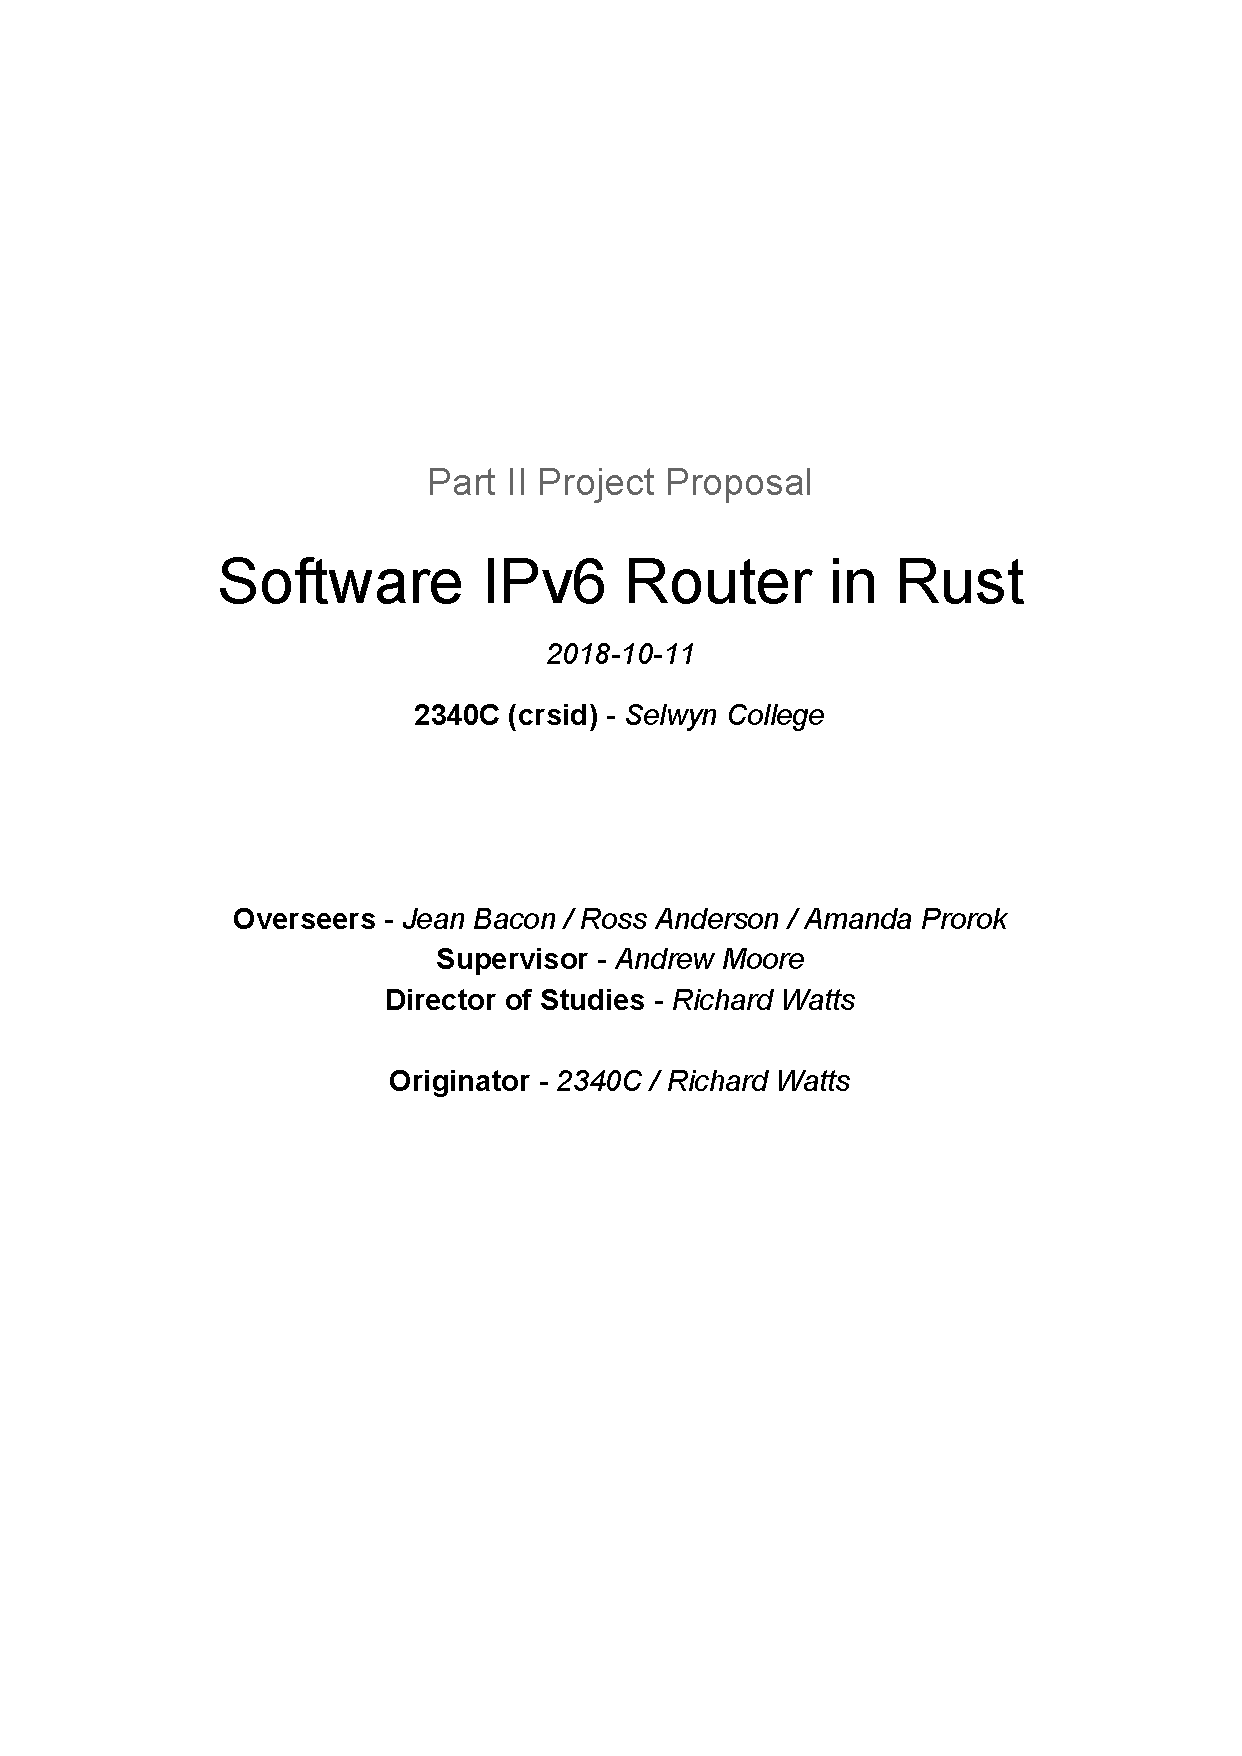
\includepdf[page=-]{proposal}

\end{document}